\documentclass[12 pt]{article}
\usepackage[utf8]{inputenc}
\usepackage{matlab-prettifier}
\usepackage[portuguese]{babel}
\usepackage{indentfirst}
\usepackage{graphicx}
\usepackage{float}
\usepackage{subcaption}
\usepackage[font=small,labelfont=bf]{caption}
\definecolor{mygreen}{RGB}{28,172,0} % color values Red, Green, Blue
\definecolor{myyellow}{rgb}{1.0, 1.0, 0.8}
\usepackage{mathtools}
\usepackage{multirow}
\usepackage{comment}
\usepackage{xcolor}
\usepackage{colortbl}
\usepackage[normalem]{ulem}               % to striketrhourhg text
\usepackage{amsmath}
\usepackage{amsfonts}
\usepackage{hyperref}
\usepackage{tcolorbox}
\usepackage{longtable}
\usepackage{enumitem}
\newcommand\redout{\bgroup\markoverwith
{\textcolor{red}{\rule[0.5ex]{2pt}{0.8pt}}}\ULon}
\renewcommand{\lstlistingname}{Código}% Listing -> Algorithm
\renewcommand{\lstlistlistingname}{Lista de \lstlistingname s}% List of Listings -> List of Algorithms

\usepackage[top=3cm,left=2cm,bottom=2cm, right=2cm]{geometry}
\usepackage{tikz}
\usetikzlibrary{decorations.pathreplacing}
\usetikzlibrary{automata}
\usetikzlibrary{positioning}
\usetikzlibrary{arrows.meta, positioning}

\usepackage{adjustbox}


% Configuração para destacar a sintaxe do Python
\lstset{ 
    language=Python,                     % A linguagem do código
    backgroundcolor=\color{myyellow}, % A cor do fundo 
    basicstyle=\ttfamily\footnotesize,   % O estilo do texto básico
    keywordstyle=\color{blue},           % Cor das palavras-chave
    stringstyle=\color{red},             % Cor das strings
    commentstyle=\color{mygreen},          % Cor dos comentários
    numbers=left,                        % Números das linhas à esquerda
    numberstyle=\tiny\color{gray},       % Estilo dos números das linhas
    stepnumber=1,                        % Número de linhas entre os números das linhas
    frame=single,                        % Moldura ao redor do código
    breaklines=true,                     % Quebra automática das linhas longas
    captionpos=t,                        % Posição da legenda
    showstringspaces=false               % Não mostra espaços em branco nas strings
    extendedchars=true,
    literate={º}{{${ }^{\underline{o}}$}}1 {á}{{\'a}}1 {à}{{\`a}}1 {ã}{{\~a}}1 {é}{{\'e}}1 {É}{{\'E}}1 {ê}{{\^e}}1 {ë}{{\"e}}1 {í}{{\'i}}1 {ç}{{\c{c}}}1 {Ç}{{\c{C}}}1 {õ}{{\~o}}1 {ó}{{\'o}}1 {ô}{{\^o}}1 {ú}{{\'u}}1 {â}{{\^a}}1 {~}{{$\sim$}}1
}


\title{%
\textbf{\huge Universidade Federal do Rio de Janeiro} \par
\textbf{\LARGE Instituto Alberto Luiz Coimbra de Pós-Graduação e Pesquisa de Engenharia} \par


\includegraphics[width=8cm]{COPPE UFRJ.png} \par

\textbf{Programa de Engenharia de Sistemas e Computação} \par

CPS767 - Algoritmos de Monte Carlo e Cadeias de Markov  \par

Prof. Daniel Ratton Figueiredo\par

\vspace{1\baselineskip}
\textbf{\textit{2ª Lista de Exercícios}} \par
}

\author{Luiz Henrique Souza Caldas\\email: lhscaldas@cos.ufrj.br}

\date{\today}

\begin{document}
\maketitle

% \tableofcontents

\section*{Questão 1: Cauda do dado}

Considere um icosaedro (um sólido Platônico de 20 faces) honesto, tal que a probabilidade associada a cada face é 1/20. Considere que o dado será lançado até que um número primo seja observado, e seja $Z$ a variável aleatória que denota o número de vezes que o dado é lançado. Responda às perguntas abaixo:

\begin{enumerate}
    \item Determine a distribuição de $Z$, ou seja $P[Z = k], k = 1, 2, \dots$. Que distribuição é esta?
    \begin{tcolorbox}[colframe=black, title=Resposta:]
        Os números primos são {2, 3, 5, 7, 11, 13, 17, 19}. Portanto, a probabilidade de obter um número primo em um lançamento é $p = \frac{8}{20} = \frac{2}{5}$. Consequentemente, a probabilidade de não obter um número primo em um lançamento é $1 - p = \frac{3}{5}$. Assim, a distribuição de $Z$ é dada por:
        $$
            \boxed{P[Z = k] = (1-p)^{k-1}p = \left(\frac{3}{5}\right)^{k-1}\left(\frac{2}{5}\right)}
        $$
        para $k = 1, 2, \dots$. Esta é uma \underline{distribuição geométrica} com parâmetro $p = \frac{2}{5}$.

    \end{tcolorbox}
    \item Utilize a desigualdade de Markov para calcular um limitante para $P[Z \geq 10]$.
    \begin{tcolorbox}[colframe=black, title=Resposta:]
        A desigualdade de Markov afirma que, para uma v.a. $Z>0$ e $a > 0$, temos:
        $$
            P[Z \geq a] \leq \frac{E[Z]}{a}
        $$
        Para calcular $E[Z]$, utilizamos a fórmula da média de uma distribuição geométrica:
        $$
            E[Z] = \frac{1}{p} = \frac{1}{\frac{2}{5}} = \frac{5}{2}
        $$
        Assim, aplicando a desigualdade de Markov com $a = 10$, obtemos:
        $$
            P[Z \geq 10] \leq \frac{E[Z]}{10} = \frac{\frac{5}{2}}{10} = \underline{\frac{1}{4} = 0.25 \quad \vline}
        $$
        Portanto, \underline{$P[Z \geq 10] \leq 0.25$}.
        Isso significa que a probabilidade de o número de lançamentos do dado ser maior ou igual a 10 é \underline{menor ou igual a 25\%}.

    \end{tcolorbox}
    \newpage
    \item Utilize a desigualdade de Chebyshev para calcular um limitante para $P[Z \geq 10]$.
    \begin{tcolorbox}[colframe=black, title=Resposta:]
    A média e variância da distribuição geométrica são $\mu = \frac{1}{p} = \frac{5}{2}$ e $\sigma^2 = \frac{1 - p}{p^2} = \frac{15}{4}$. Aplicando Chebyshev:
    $$
    P[|Z - \mu| \geq k \sigma] \leq \frac{1}{k^2}
    $$
    Subtraindo $\mu$ de ambos os lados em  $P[Z \geq 10]$, temos:
    $$
    P[Z \geq 10] = P[Z - \mu \geq 10 - \tfrac{5}{2}] = P[Z - \mu \geq \tfrac{15}{2}] \leq P[|Z - \mu| \geq k \sigma]
    $$

    Fazendo $k \sigma = \tfrac{15}{2}$, então 
    $$k = \frac{15}{2} \cdot \frac{2}{\sqrt{15}} = \sqrt{15}$$
    
    Assim, temos:
    $$
    \boxed{P[Z \geq 10] \leq \frac{1}{15} \approx 0.0667}
    $$
    \end{tcolorbox}

    \item Calcule o valor exato de $P[Z \geq 10]$ (dica: use probabilidade complementar). Compare os valores obtidos.
    \begin{tcolorbox}[colframe=black, title=Resposta:]
    $$
    P[Z \geq 10] = 1 - P[Z \leq 9] = 1 - \sum_{k=1}^9 P[Z = k]
    $$
    $$
    P[Z \geq 10] = 1 - \frac{2}{5} \sum_{k=1}^9 \left(\frac{3}{5}\right)^{k-1} = 1 - \frac{2}{5} \cdot \frac{1 - \left(\frac{3}{5}\right)^9}{1 - \frac{3}{5}} = \left(\frac{3}{5}\right)^9
    $$
    $$
    \boxed{P[Z \geq 10] = \left(\frac{3}{5}\right)^9 \approx 0{,}0101}
    $$

    Comparando os valores:
    \begin{itemize}
        \item Markov: $P[Z \geq 10] \leq 0{,}25$
        \item Chebyshev: $P[Z \geq 10] \leq 0{,}0667$
        \item Valor exato: $P[Z \geq 10] \approx 0{,}0101$
    \end{itemize}
    Ambas as desigualdades fornecem limites conservadores, sendo Chebyshev mais ajustado que Markov. O valor exato é o mais preciso.
    \end{tcolorbox}

\end{enumerate}

\section*{Questão 2: Pesquisa eleitoral}

Você leu no jornal que uma pesquisa eleitoral com 1500 pessoas indicou que 40\% dos entrevistados prefere o candidato A enquanto 60\% preferem o candidato B. Determine a margem de erro desta pesquisa usando uma confiança de 95\%. O que você precisou assumir para calcular a margem de erro?
\begin{tcolorbox}[colframe=black, title=Resposta:]
    Seja $X_i$ uma variável aleatória i.i.d. que representa a preferência do entrevistado $i$, com:
    $$
    X_i = \begin{cases}
    1 & \text{se prefere o candidato A} \\
    0 & \text{se prefere o candidato B}
    \end{cases}
    $$
    
    A média amostral de $X_i$ é dada por:
    $$
    M_n = \frac{1}{n}\sum_{i=1}^n X_i =  0.4
    $$

    Como $E[M_n] = \mu$, onde $\mu=p$ é a média da distribuição de Bernoulli, temos, pela desigualdade de Chebyshev:
    $$
    P[|M_n - p| \geq k \sigma_{M_n}] \leq \frac{1}{k^2}
    $$
    onde $\sigma_{M_n} = \sqrt{\frac{\sigma^2}{n}}$ é o desvio padrão da média amostral, sendo $\sigma^2 = p(1-p)$ a variância da distribuição de Bernoulli.

    Fazendo a margem de erro $\epsilon = k \sigma_{M_n}$, temos:
    $$
    k=\frac{\epsilon}{\sigma_{M_n}} = \frac{\epsilon\sqrt{n}}{\sigma} \Rightarrow P[|M_n - p| \geq \epsilon] \leq \frac{\sigma^2}{\epsilon^2n}
    $$

    Aplicando o complementar, temos:
    $$
    P[|M_n - p| < \epsilon] = 1 - P[|M_n - p| \geq \epsilon] \geq 1 - \frac{\sigma^2}{\epsilon^2n}=\beta
    $$
    onde $\beta$ é o nível de confiança que queremos.

    Resolvendo para $\epsilon$:
    $$
    \epsilon = \sqrt{\frac{\sigma^2}{(1-\beta)n}} = \sqrt{\frac{p(1-p)}{(1-\beta)n}}
    $$

    Assumindo que $n$ é grande o suficiente para $M_n=\mu=p=0.4$, temos:
    $$
    \epsilon = \sqrt{\frac{0.4(1-0.4)}{(1-0.95)1500}} = \sqrt{\frac{0.4(0.6)}{0.05\cdot1500}} = \sqrt{\frac{0.24}{75}} = \sqrt{0.0032} \approx \underline{0.0565 \quad \vline}
    $$
\end{tcolorbox}

\section*{Questão 3: Sanduíches}

Você convidou 64 pessoas para uma festa e agora precisa preparar sanduíches para os convidados. Você acredita que cada convidado irá comer 0, 1 ou 2 sanduíches com probabilidades 1/4, 1/2 e 1/4, respectivamente. Assuma que o número de sanduíches que cada convidado irá comer é independente de qualquer outro convidado. Quantos sanduíches você deve preparar para ter uma confiança de 95\% de que não vai faltar sanduíches para os convidados?
\begin{tcolorbox}[colframe=black, title=Resposta:]
    Seja $X_i$ a variável aleatória que representa o número de sanduíches que o convidado $i$ irá comer, com distribuição de probabilidade dada por:
    $$
    p_i = \begin{cases}
    \frac{1}{4} & \text{se } i=0 \\
    \frac{1}{4} & \text{se } i=1 \\
    \frac{1}{4} & \text{se } i=2 \\
    \end{cases}
    $$

    O valor esperado de $X_i$ é dado por:
    $$
    E[X_i] = \sum_{i=0}^2 i \cdot p_i = 0 \cdot \frac{1}{4} + 1 \cdot \frac{1}{2} + 2 \cdot \frac{1}{4} = 0 + \frac{1}{2} + \frac{2}{4} = 1
    $$

    A variância de $X_i$ é dada por:
    $$
    E[X_i^2] = \sum_{i=0}^2 i^2 \cdot p_i = 0^2 \cdot \frac{1}{4} + 1^2 \cdot \frac{1}{2} + 2^2 \cdot \frac{1}{4} = 0 + \frac{1}{2} + \frac{4}{4} = 0 + \frac{1}{2} + 1 = \frac{3}{2}
    $$
    $$
    Var[X_i] = E[X_i^2] - (E[X_i])^2 = \frac{3}{2} - 1^2 = \frac{3}{2} - 1 = \frac{1}{2}
    $$


\end{tcolorbox}

\section*{Questão 4: Graus improváveis}

Considere o modelo de grafo aleatório de Erdős-Rényi (também conhecido por $G(n, p)$), onde cada possível aresta de um grafo rotulado com $n$ vértices ocorre com probabilidade $p$, independentemente. Responda às perguntas abaixo:

\begin{enumerate}
    \item Determine a distribuição do grau do vértice 1 (em função de $n$ e $p$).
    \begin{tcolorbox}[colframe=black, title=Resposta:]

    \end{tcolorbox}
    \item Determine o valor $\gamma$ (em função de $n$ e $p$) tal que com alta probabilidade ($1 - 1/n$) o grau observado no vértice 1 é menor ou igual a $\gamma$.
    \begin{tcolorbox}[colframe=black, title=Resposta:]

    \end{tcolorbox}
\end{enumerate}

\section*{Questão 5: Calculando uma importante constante}

Seja $X_i$ uma sequência i.i.d. de v.a. contínuas uniformes em $[0, 1]$. Seja $V$ o menor número $k$ tal que a soma das primeiras $k$ variáveis seja maior do que 1. Ou seja, $V = \min\{k \mid X_1 + \cdots + X_k \geq 1\}$.

\begin{enumerate}
    \item Escreva e implemente um algoritmo para gerar uma amostra de $V$.
    \begin{tcolorbox}[colframe=black, title=Resposta:]
        \begin{itemize}
            \item Pseudo-código:
            \begin{verbatim}
    soma = 0;
    contador = 0;
    enquanto soma < 1 faça
        x = amostra de U[0, 1];
        soma = soma + x;
        contador = contador + 1;
    retorne contador;
            \end{verbatim}
            \item Implementação em Python:
            \begin{lstlisting}[language=Python]
    def amostra_V():
        soma = 0
        contador = 0
        while soma < 1:
            x = random()
            soma += x
            contador += 1
        return contador
            \end{lstlisting}
        \end{itemize}
    \end{tcolorbox}
    \item Escreva e implemente um algoritmo de Monte Carlo para estimar o valor esperado de $V$.
    \begin{tcolorbox}[colframe=black, title=Resposta:]
        \begin{itemize}
            \item Definição do estimador:
            Pela Lei dos Grandes Números, temos que, para $n$ suficientemente grande, a média amostral converge para o valor esperado:
            $$
            E[V] \approx \frac{1}{n} \sum_{i=1}^n V_i
            $$
            onde $V_i$ é a amostra de $V$ obtida na iteração $i$.
            \item Pseudo-código:
            \begin{verbatim}
    n = N; // número de amostras
    soma = 0;
    para i = 1 até n faça
        soma = soma + amostra_V();
    estimador = soma / n;
    retorne estimador;
            \end{verbatim}
            \item Implementação em Python:
            \begin{lstlisting}[language=Python]
    def estimador_E(n):
        soma = 0
        for i in range(n):
            x = amostra_V()
            soma += x
        return soma / n
            \end{lstlisting}
        \end{itemize}
    \end{tcolorbox}
    \item Trace um gráfico do valor estimado em função do número de amostras. Para qual valor seu estimador está convergindo?
    \begin{tcolorbox}[colframe=black, title=Resposta:]
        Código para gerar o gráfico:
        \begin{lstlisting}[language=Python]
    def grafico_E(n_max):
    
        n_values = list(range(1, n_max + 1))
        E_values = [estimador_E(n) for n in n_values]

        plt.plot(n_values, E_values, label='E[V] a cada n')
        label = f'Limite E[V] = {E_values[-1]}'
        plt.axhline(y=E_values[-1], color='r', linestyle='--', label=label)
        plt.title('Estimador de E[V] em função de n')
        plt.xlabel('n')
        plt.ylabel('E[V]')
        plt.grid(True)
        plt.legend()
        plt.show()
        \end{lstlisting}
        Para $10^4$ amostras, o estimador converge para aproximadamente $E[V] \approx 2.7076$, como visto na figura abaixo.
    \end{tcolorbox}

    \begin{figure}[H]
        \centering
        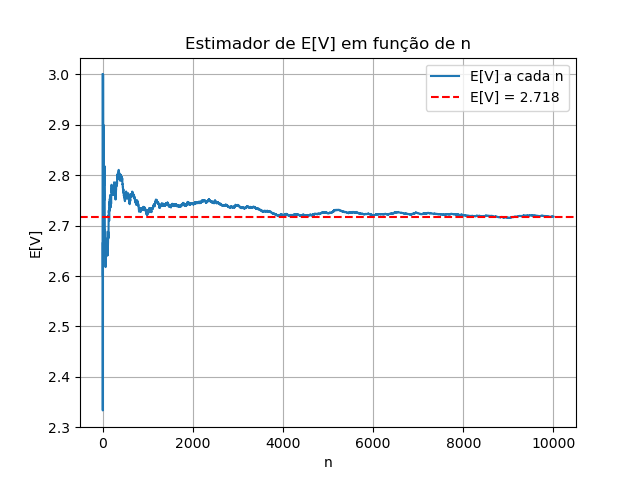
\includegraphics[width=0.8\textwidth]{q5_3.png}
        \caption{Estimador de $E[V]$ em função de $n$}
        \label{fig:estimador_E}
    \end{figure}
\end{enumerate}

\section*{Questão 6: Transformada inversa}

Mostre como o método da transformada inversa pode ser usado para gerar amostras de uma v.a. contínua $X$ com as seguintes distribuições:

\begin{enumerate}
    \item Distribuição exponencial com parâmetro $\lambda > 0$, cuja função densidade é dada por $f_X(x) = \lambda e^{-\lambda x}$, para $x \geq 0$.
    \begin{tcolorbox}[colframe=black, title=Resposta:]

    \end{tcolorbox}
    \item Distribuição de Pareto com parâmetros $x_0 > 0$ e $\alpha > 0$, cuja função densidade é dada por $f_X(x) = \frac{\alpha x_0^\alpha}{x^{\alpha + 1}}$, para $x \geq x_0$.
    \begin{tcolorbox}[colframe=black, title=Resposta:]

    \end{tcolorbox}
\end{enumerate}

\section*{Questão 7: Contando domínios na Web}

Quantos domínios web existem dentro da UFRJ? Mais precisamente, quantos domínios existem dentro do padrão de nomes \texttt{http://www.[a-z](k).ufrj.br}, onde $[a-z](k)$ é qualquer sequência de caracteres de comprimento $k$ ou menor? Construa um algoritmo de Monte Carlo para estimar este número.

\begin{enumerate}
    \item Descreva a variável aleatória cujo valor esperado está relacionado com a medida de interesse. Relacione analiticamente o valor esperado com a medida de interesse.
    \begin{tcolorbox}[colframe=black, title=Resposta:]

    \end{tcolorbox}
    \item Implemente o método de Monte Carlo para gerar amostras e estimar a medida de interesse. Para determinar o valor de uma amostra, você deve consultar o domínio gerado para determinar se o mesmo existe (utilize uma biblioteca web para isto).
    \begin{tcolorbox}[colframe=black, title=Resposta:]

    \end{tcolorbox}
    \item Assuma que $k = 4$. Seja $\hat{w}_n$ o valor do estimador do número de domínios após $n$ amostras. Trace um gráfico em escala semi-log (eixo-$x$ em escala log) de $\hat{w}_n$ em função de $n$ para $n = 1, \dots, 10^5$ (ou mais, se conseguir). O que você pode dizer sobre a convergência de $\hat{w}_n$?
    \begin{tcolorbox}[colframe=black, title=Resposta:]

    \end{tcolorbox}
\end{enumerate}

\section*{Questão 8: Rejection Sampling}

Considere o problema de gerar amostras de uma v.a. $X \sim \text{Binomial}(1000, 0.2)$.

\begin{enumerate}
    \item Descreva uma proposta simples de função de probabilidade para gerar amostras de $X$ usando Rejection Sampling. Calcule a eficiência dessa proposta.
    \begin{tcolorbox}[colframe=black, title=Resposta:]

    \end{tcolorbox}
    \item Lembrando que a distribuição Binomial tem a forma de sino, centrada em sua média, proponha outra função de probabilidade para gerar amostras de $X$ usando Rejection Sampling. Calcule a eficiência dessa proposta e compare com a eficiência acima. O que você pode concluir?
    \begin{tcolorbox}[colframe=black, title=Resposta:]

    \end{tcolorbox}
\end{enumerate}

\section*{Questão 9: Integração de Monte Carlo e Importance Sampling}

Considere a função $g(x) = e^{-x^2}$ e a integral de $g(x)$ no intervalo $[0, 1]$.

\begin{enumerate}
    \item Implemente um método de Monte Carlo simples para estimar o valor da integral.
    \begin{tcolorbox}[colframe=black, title=Resposta:]

    \end{tcolorbox}
    \item Intuitivamente, muitas amostras de $g(x)$ vão ter valores muito baixos. Dessa forma, utilize Importance Sampling para melhorar a qualidade do estimador do valor da integral. Em particular, utilize a função de densidade $h(x) = Ae^{-x}$ definida em $[0, 1]$ onde $A$ é o valor da constante de normalização. Mostre como gerar amostras de $h(x)$.
    \begin{tcolorbox}[colframe=black, title=Resposta:]

    \end{tcolorbox}
    \item Compare os dois métodos. Trace um gráfico do erro relativo de cada um dos estimadores em função do número de amostras. Ou seja, $|\hat{I}_n - I|/I$ onde $I$ é o valor exato da integral e $\hat{I}_n$ é o valor do estimador com $n$ amostras, para $n = 10^1, 10^2, \dots, 10^6$.
    \begin{tcolorbox}[colframe=black, title=Resposta:]

    \end{tcolorbox}
\end{enumerate}


\section*{Códigos}

Os códigos utilizados para a resolução dos exercícios estão disponíveis no repositório do GitHub: \url{https://github.com/lhscaldas/CPS767_MCMC/}

% \bibliographystyle{abntex2-num} % Escolha o estilo de citação desejado
% \nocite{sutton2018reinforcement}
% \bibliography{bibliografia} % Nome do arquivo .bib (sem a extensão)

\end{document}